% Options for packages loaded elsewhere
\PassOptionsToPackage{unicode}{hyperref}
\PassOptionsToPackage{hyphens}{url}
%
\documentclass[
]{book}
\usepackage{lmodern}
\usepackage{amssymb,amsmath}
\usepackage{ifxetex,ifluatex}
\ifnum 0\ifxetex 1\fi\ifluatex 1\fi=0 % if pdftex
  \usepackage[T1]{fontenc}
  \usepackage[utf8]{inputenc}
  \usepackage{textcomp} % provide euro and other symbols
\else % if luatex or xetex
  \usepackage{unicode-math}
  \defaultfontfeatures{Scale=MatchLowercase}
  \defaultfontfeatures[\rmfamily]{Ligatures=TeX,Scale=1}
\fi
% Use upquote if available, for straight quotes in verbatim environments
\IfFileExists{upquote.sty}{\usepackage{upquote}}{}
\IfFileExists{microtype.sty}{% use microtype if available
  \usepackage[]{microtype}
  \UseMicrotypeSet[protrusion]{basicmath} % disable protrusion for tt fonts
}{}
\makeatletter
\@ifundefined{KOMAClassName}{% if non-KOMA class
  \IfFileExists{parskip.sty}{%
    \usepackage{parskip}
  }{% else
    \setlength{\parindent}{0pt}
    \setlength{\parskip}{6pt plus 2pt minus 1pt}}
}{% if KOMA class
  \KOMAoptions{parskip=half}}
\makeatother
\usepackage{xcolor}
\IfFileExists{xurl.sty}{\usepackage{xurl}}{} % add URL line breaks if available
\IfFileExists{bookmark.sty}{\usepackage{bookmark}}{\usepackage{hyperref}}
\hypersetup{
  pdftitle={Coupling Groundwater Vulnerability to Contamination and Extreme Precipitation Events Using Active and Passive Remote Sensing Data Products},
  pdfauthor={Andrew Murray},
  hidelinks,
  pdfcreator={LaTeX via pandoc}}
\urlstyle{same} % disable monospaced font for URLs
\usepackage{longtable,booktabs}
% Correct order of tables after \paragraph or \subparagraph
\usepackage{etoolbox}
\makeatletter
\patchcmd\longtable{\par}{\if@noskipsec\mbox{}\fi\par}{}{}
\makeatother
% Allow footnotes in longtable head/foot
\IfFileExists{footnotehyper.sty}{\usepackage{footnotehyper}}{\usepackage{footnote}}
\makesavenoteenv{longtable}
\usepackage{graphicx,grffile}
\makeatletter
\def\maxwidth{\ifdim\Gin@nat@width>\linewidth\linewidth\else\Gin@nat@width\fi}
\def\maxheight{\ifdim\Gin@nat@height>\textheight\textheight\else\Gin@nat@height\fi}
\makeatother
% Scale images if necessary, so that they will not overflow the page
% margins by default, and it is still possible to overwrite the defaults
% using explicit options in \includegraphics[width, height, ...]{}
\setkeys{Gin}{width=\maxwidth,height=\maxheight,keepaspectratio}
% Set default figure placement to htbp
\makeatletter
\def\fps@figure{htbp}
\makeatother
\setlength{\emergencystretch}{3em} % prevent overfull lines
\providecommand{\tightlist}{%
  \setlength{\itemsep}{0pt}\setlength{\parskip}{0pt}}
\setcounter{secnumdepth}{5}
\usepackage{booktabs}
\usepackage[]{natbib}
\bibliographystyle{apalike}

\title{Coupling Groundwater Vulnerability to Contamination and Extreme Precipitation Events Using Active and Passive Remote Sensing Data Products}
\author{Andrew Murray}
\date{2020-02-10}

\begin{document}
\maketitle

{
\setcounter{tocdepth}{1}
\tableofcontents
}
\hypertarget{overview}{%
\chapter{Overview}\label{overview}}

\hypertarget{abstract}{%
\section{Abstract}\label{abstract}}

In the past five years, twenty tropical cyclones have made landfall in the southeastern United States, many with devastating impacts and particularly in areas that are heavily dependent on groundwater. Geophysical landscape features, temporal variability of soil moisture, and land cover are major drivers of groundwater vulnerability to contamination. Extreme precipitation events such as tropical cyclones overwhelm and impose changes to each of these variables in measurable ways. Investigating the relationships and the ways in which to measure these impacts will enable future forecasting of vulnerability and better inform disaster response efforts, directly and positively affecting human health.
The factors most closely associated with a person's view of their water quality is taste followed by odor and color. Many contaminants can exist in levels low enough to have no effect on taste, odor or color but orders of magnitude higher than may be damaging to human health. Groundwater vulnerability has been successfully estimated using the DRASTIC method but has been limited by a lack of continuous soil moisture inputs for required hydrogeological variables. Soil moisture typically requires data to be physically collected in the field. However, recent advances in satellite remote sensing have yielded global high-resolution soil moisture maps every 1-3 days. Along with publicly available data, this soil moisture data can be used to create inputs for an improved groundwater vulnerability index which will allow us to estimate the vulnerability to groundwater resources following extreme precipitation events such as tropical cyclones. Estimates will be calculated for twenty tropical cyclones, which have hit the southeastern United States since June, 2015. Water quality tests, collected from groundwater wells, which were collected following multiple cyclones will be used to validate estimates in order to accurately produce a predictive model usable for future extreme precipitation events. This research will yield a direct benefit to human health, cyclone preparation and response while informing government agencies and emergency responders.

\hypertarget{committee-composition}{%
\section{Committee Composition}\label{committee-composition}}

\begin{itemize}
\tightlist
\item
  \href{http://diegori.web.unc.edu/}{Dr.~Diego Riveros-Iregui}*†
\item
  \href{https://waterpotential.wordpress.ncsu.edu/}{Dr.~Ryan Emannuel}♠
\item
  \href{http://cekd.web.unc.edu/}{Dr.~Charles Konrad}†
\item
  \href{http://aaron.web.unc.edu/}{Dr.~Aaron Moody}†
\item
  \href{http://csong.web.unc.edu/}{Dr.~Conghe Song}†
\end{itemize}

* Chair
† University of North Carolina - Chapel Hill
♠ North Carolina State University

\hypertarget{intro}{%
\chapter{Introduction}\label{intro}}

~~~~~~In the past five years, twenty tropical cyclones have made landfall in the southeastern United States, many with devastating impacts in areas that are heavily dependent on groundwater. In 2016, Hurricane Matthew broke more than 14 peak streamflow records, drowning thousands of hogs and millions of chickens and turkeys while overwhelming waste lagoons that spilled into local waterways that reached groundwater systems (\citet{robbins2016} \& \citet{porter2017}). More than 2,200 community water systems and over 1,700 wastewater facilities were compromised by Hurricane Harvey in 2017, including a reported half-billion-gallon spill of industrial wastewater which mixed with storm water and surged out of a single chemical plant \citep{bajak2018}. In 2018, Hurricanes Florence and Michael collectively impacted Florida, Alabama, Georgia, the Carolinas and Virginia, bringing new examples of floodwaters that continued to rise well after the rains had ended, compromising hog and poultry farms, chemical plants, and vast expanses of agricultural areas. Tropical Storm Imelda (2019) dropped up to 950 mm of rain in some areas \citep{R-prism}, showing that devastating flooding is not limited to those storms labeled as `hurricanes.' In fact, most of the coastal southeastern United States has experienced intense rainfall from a tropical cyclone at least once in the past five years \protect\hyperlink{fig:ppt}{Figure \ref{fig:ppt}}. In the aftermath of extreme precipitation events, emergency responders, or researchers, often provide free or discounted water testing to well owners. While public water utilities are required to conduct regular testing of water supplies by the Safe Drinking Water Act (SDWA), private water supplies are not protected under the SDWA and are therefore not subject to testing requirements; they are thus more susceptible to undetected contamination of drinking water. Consequently, the burden of testing drinking water falls on the homeowner or tenant who may not suspect that their water has been contaminated. The factors most closely associated with a person's judgment of their water quality are taste followed by odor and color \citep{defranca2010}, but many contaminants are known to pose serious threats to human health at levels low enough to have no effect on taste, odor, or color. For example, benzene, a carcinogenic component of gasoline, has an EPA Maximum Contaminant Level (MCL) of .005 mg/L and a residence time in groundwater approaching thirty years \citep{molson2002}. Consequently, it is important to understand and assess groundwater vulnerability without depending on the information provided by individual homeowners.

\begin{figure}
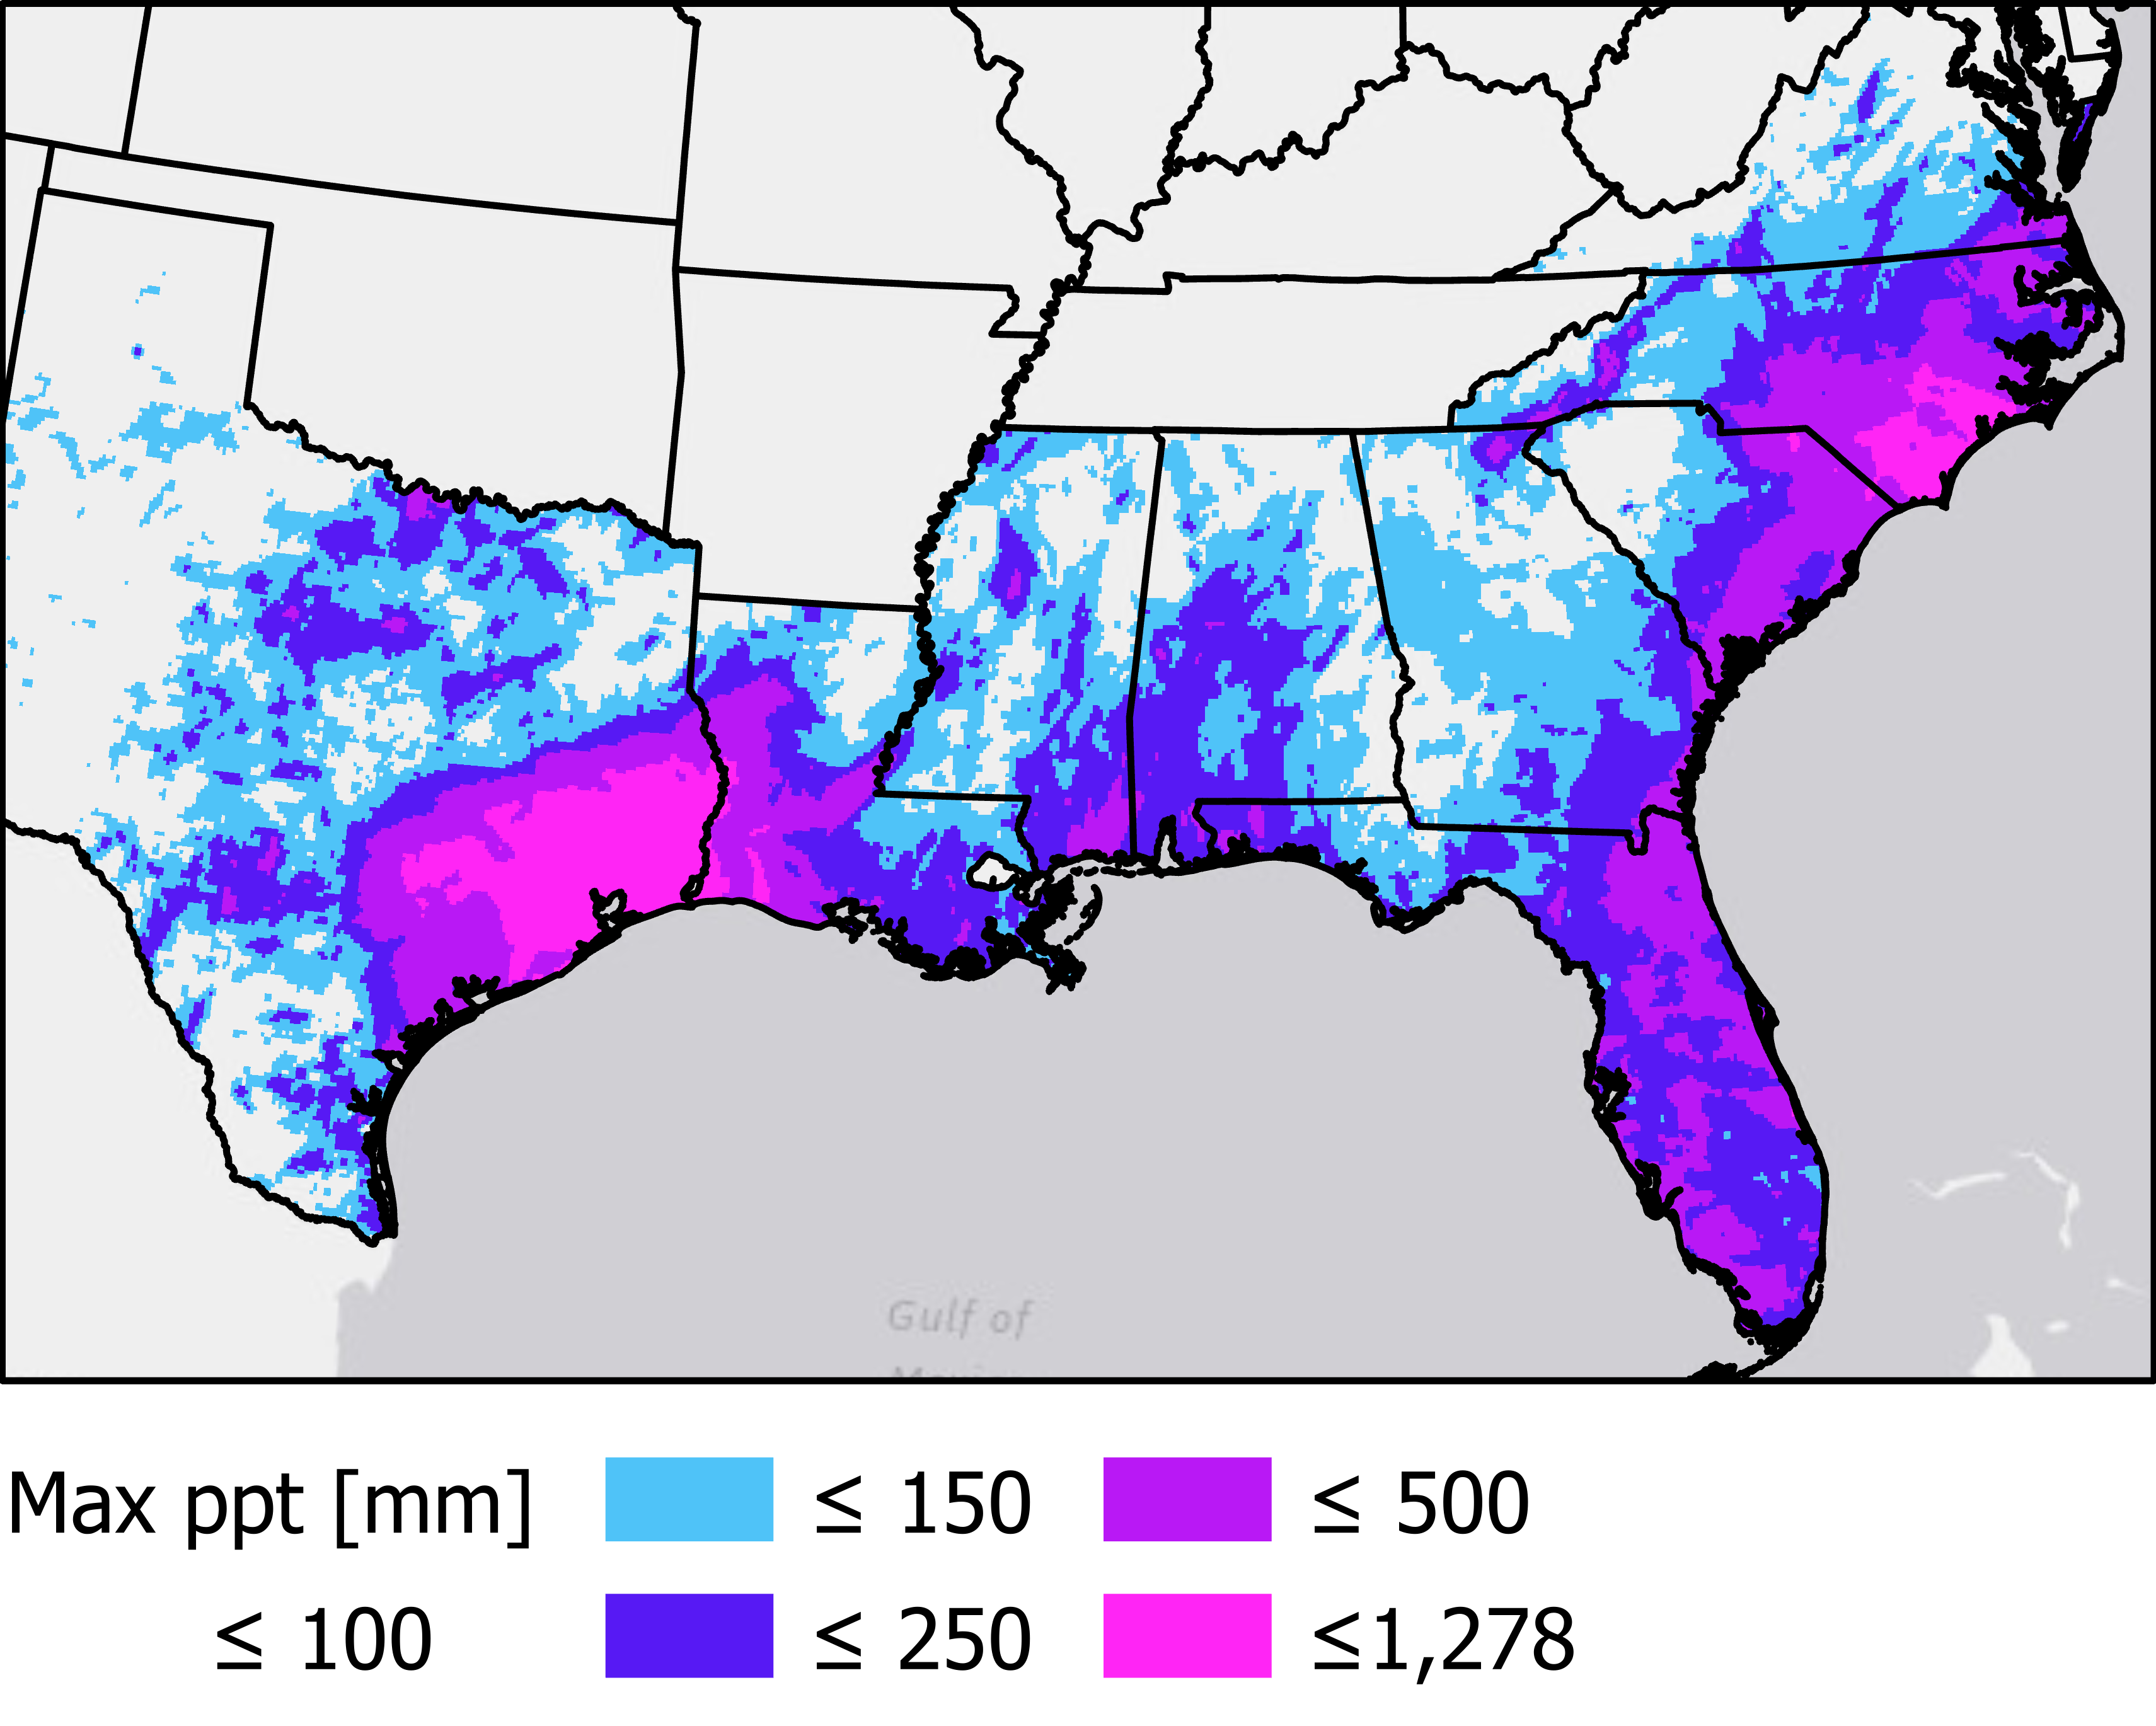
\includegraphics[width=47.51in]{img/max_ppt} \caption{Maximum precipitation greater than 100 mm experienced during a single tropical cyclone event since the start of the 2015 tropical cyclone season.}\label{fig:ppt}
\end{figure}

Currently, we have no way of estimating groundwater vulnerability to contamination following extreme precipitation events. Reports in the aftermath of Hurricane Matthew showed that soil saturation and precipitation in the 45 days prior to the storm amplified peak stream flows and the inundation extent during and after the storm\citep{musser2017}. It should be noted that while the bulk of attention is given to major hurricanes, there is no correlation between wind speed (storm category) and either precipitation intensity or mean precipitation over land \protect\hyperlink{fig:stormPts}{Figure \ref{fig:stormPts}}. Analytical complications are introduced by variability in land cover, which is known to directly affect soil water infiltration rates during and after rainfall events. In urban areas with variable density of impervious surface cover, infiltration rates can vary by up to 60\% over small spatial scales\citep{pauleit2000}, while in undeveloped land infiltration rates can vary between \textless{} .1 to \textgreater{} 10 m / day\citep{bouwer1999}. I seek to provide quantitative understanding of the vulnerability of groundwater resources to contamination during and after extreme precipitation events, using temporal changes in soil moisture (SM) in the days prior to and following an event and in combination with land use/land cover information. My research will utilize both passive and active satellite based and sub-orbital airborne sensors, in conjunction with established sources of geologic and atmospheric information.

\begin{figure}
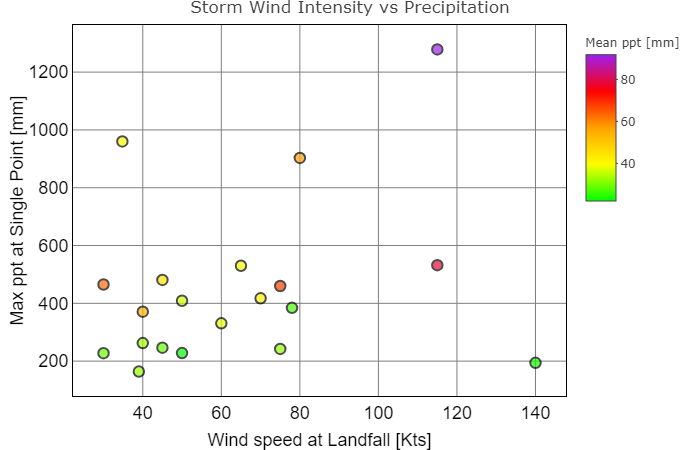
\includegraphics[width=1\linewidth]{img/stormPts} \caption{Wind speed at landfall plotted against maximum total rainfall experienced at a single point per cyclone event and colored by average mean precipitation experienced over the impacted land area }\label{fig:stormPts}
\end{figure}

I propose to utilize L, C and X band sensors producing SM data in combination with land cover and a tried-and-true groundwater vulnerability indexing method to predict groundwater areas prone to contact with surface waters, and thus predict those most vulnerable to contamination from extreme events. My previous work at the Environmental Protection Agency (EPA) has shown that North Carolina, Florida, and Texas have the first, second, and fifth highest populations served by private domestic groundwater wells in the nation, respectively\citep{murray2020}. More than five million privately owned wells have been impacted by tropical cyclones since 2015 \protect\hyperlink{fig:pptWellsBar}{Figure \ref{fig:pptWellsBar}}. The Southeastern U.S. has high reliance on private water supplies, yet also displays heterogenous land use types and varying physical landscapes. For example, Houston is characterized by heavily urbanized and industrial landscapes, largely dominated by the oil and gas sector. The Florida coast represents low lying wetland landscapes heavily susceptible to groundwater contamination due to the prevalence of limestone. The eastern Carolinas are characterized by mixed rural and urban landscapes with a large portion of the economy built on agriculture, specifically intensive hog and poultry farming, highlighting the risk for agricultural contaminants to reach groundwater systems.\\

\begin{figure}
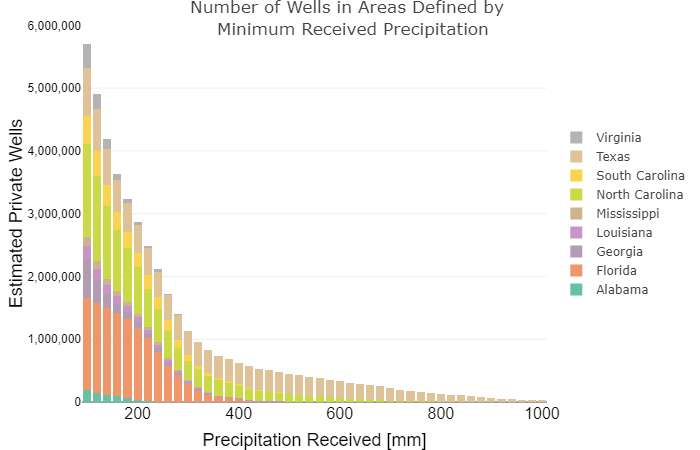
\includegraphics[width=1\linewidth]{img/pptWellsBar} \caption{Estimated private wells in areas impacted by greater than 100mm of precipitation in a single event. Only tropical cyclonic events since 2015 considered here.}\label{fig:pptWellsBar}
\end{figure}

With recent developments in remotely sensed SM data products from multiple active and passive sensors using L, C and X bands, it is possible to create global coverage SM maps with high spatial resolution\citep{mohanty2017}. This information can be used to evaluate the temporal variability in hydraulic parameters such as conductivity and water retention(\citet{ahuja1993} \& \citet{chen1993}). The SM Active Passive (SMAP) satellite, equipped with a radiometer for passive L band (40 km2 resolution) and C band radar is used to produce a Level 4 SM data product (9 km resolution) quantifying daily SM measurements\citep{reichle2017}. Although the C band radar on SMAP failed two months after launch, recent work has been completed to assimilate the SMAP passive radiometer with Sentinel 1A and 1B active radar data (\citet{das2018} \& \citet{santi2018}), which is shown to outperform SMAP passive data alone when compared to in situ data measurements \citep{lievens2017}.

\hypertarget{hypothesis}{%
\chapter{Hypothesis}\label{hypothesis}}

~~~~~~Extreme precipitation events inundate areas with water so quickly that landscapes are unable to drain the excess water. This flash of water inundation leads to the mobilization of contaminants and provides pathways for those contaminants to enter groundwater. For example, 68\% of waterborne disease outbreaks in the United States between 1948 and 1998 were immediately preceded by precipitation events above the 80th percentile, with a two-month lag in groundwater \citep{curriero2001}. I hypothesize that groundwater storage availability is directly related to how landscapes respond to extreme precipitation. For example, if available groundwater storage is low (i.e., if soil is near saturation) prior to an extreme precipitation event, the landscape cannot effectively offset the impacts of an excess amount of water. Conversely, if available groundwater storage is high (i.e., if soil is dry), the landscape can more readily mitigate the impact of an extreme precipitation event.

~~~~~~Geophysical landscape features, temporal variability of SM, and land cover are major drivers of groundwater vulnerability to contamination. Extreme precipitation events, such as tropical cyclones, overwhelm and impose changes to each of these variables in measurable ways. My preliminary analysis suggests that landscapes respond to extreme precipitation differently relative to land cover patterns \protect\hyperlink{fig:boxPlot}{Figure \ref{fig:boxPlot}} and available groundwater storage leading up to an extreme event. Investigating the relationships and the ways in which to measure these impacts will enable future forecasting of vulnerability and better inform disaster response efforts, directly and positively affecting public health.

\begin{figure}
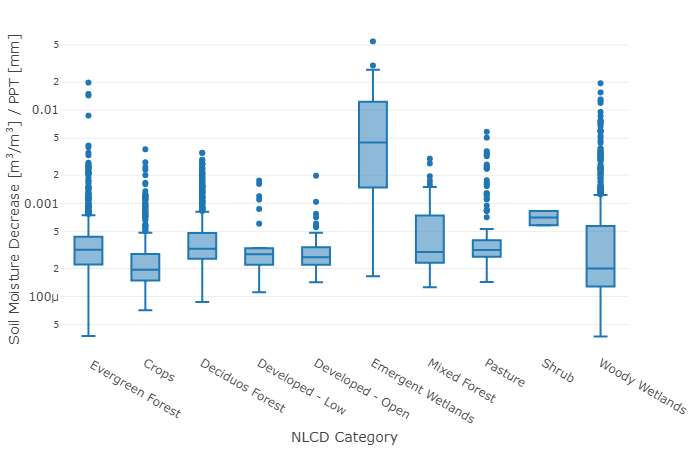
\includegraphics[width=1\linewidth]{img/boxplot} \caption{Drop in soil moisture following Hurricane Florence normalized by amount of precipitation and categorized by National Landcover Dataset classification}\label{fig:boxPlot}
\end{figure}

\hypertarget{methods}{%
\chapter{Methods}\label{methods}}

~~~~~~I will start with an established groundwater vulnerability index and update it using SM products, precipitation, landcover, and LAI, while also leveraging new technologies to supply dynamic hydrogeological data to better calibrate existing variables. I will evaluate the SMAP L4 Surface and Root Zone SM (9 km), SMAP/Sentinel-1 L2 Radiometer/Radar SM data (3 km) and SMAP Enhanced L3 Radiometer Daily SM (9 km) products for use within this new, dynamic vulnerability index. Changes in LAI will be assessed pre- and post-event to determine changes in permeability values utilizing accepted methods leveraging MODIS data \citep{song2013optical}. LCLU will also be considered via the National Land Cover Dataset. This information will be used to parameterize a DRASTIC vulnerability index \citep{aller1985}, amply used in hydrological research (\citet{hamza2006}, \citet{jang2017}, \citet{panagopoulos2006}, \citet{remesan2008}, \citet{rundquist1991}, \citet{uddameri2007}). DRASTIC is a ranking scheme that uses a combination of weights consisting of \textbf{D}epth to water table, net \textbf{R}echarge, \textbf{A}quifer media, \textbf{S}oil media, \textbf{T}opography, \textbf{I}mpact of the vadose zone, and hydraulic \textbf{C}onductivity of the aquifer. A spatially distributed DRASTIC index will be calculated using static variables which are readily available and updated using land cover and daily parameters calculated from remotely sensed SM data. Results will be assessed to characterize the spatial variability of vulnerability of groundwater systems surrounding extreme precipitation events.

~~~~~~Currently, the best method for estimating SM at an optimal combination of spatial and temporal resolution is the SMAP L4 Global 3-hourly 9 km group of products which show that while the patterns of SM increase closely align with precipitation, landscape is much more spatially complex \protect\hyperlink{fig:florence}{Figure \ref{fig:florence}}. The SMAP/Sentinel L2 3km SM product which further refines spatial resolution and enhance forecasting ability \citep{das2018}, but comes at the cost of temporal resolution. The newer L2 3km assimilated product yields global coverage every \textasciitilde12 days as opposed to every 1.5 days for 9km data. Multiple SM measurements will be used to cross validate SMAP data such as NASA's Uninhabited Aerial Vehicle Synthetic Aperture Radar (UAVSAR) mission, which was flown multiple times following Hurricane Harvey over Houston and Hurricane Florence over the Carolinas. These data will aid in validating models of SM response across various land cover types post-storm by measuring performance against the SMAP/Sentinel data products as inputs to the groundwater vulnerability index. Additionally, this work will leverage and complement the SM Viewer (SMV) maintained by NASA's Oak Ridge National Laboratory Distributed Data Archive Center, which collects available SM data from a variety of remotely sensed and in-situ sources \citep{shrestha2019}.

\begin{figure}
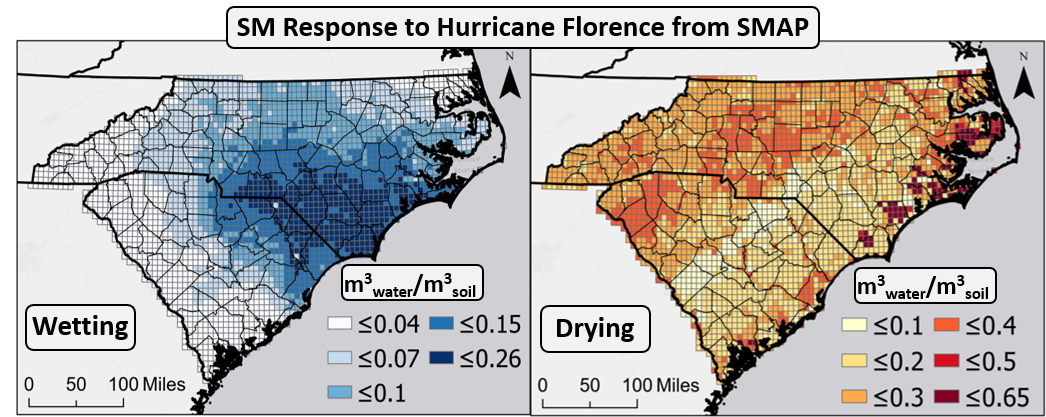
\includegraphics[width=1\linewidth]{img/florence} \caption{The SMAP 3-Hourly 9-km root zone SM product shows increase (wetting) in SM from pre-landfall to peak and the following decrease (drying) in SM from peak to low, in the three weeks after landfall of Hurricane Florence. Note spatial differences between both images}\label{fig:florence}
\end{figure}

~~~~~~The DRASTIC index, developed in 1987 by the National Groundwater Well Association and U.S. EPA heavily realies on subsurface geologic variables and typically uses data collected over extended periods of time to calculate `normal' index values for a specific location. Groundwater vulnerability, however, is not static and can fluctuate depending on current conditions relating to saturation level of the soil, seasonality, weather conditions and land cover. An improvement upon the DRASTIC index is needed to understand how vulnerability fluctuates prior and in response to extreme weather events in order to estimate regions vulnerable to groundwater contamination and to better inform the public, emergency response efforts and future research.

~~~~~~Input data for aquifer and soil media, topography, and vadose zone impact are available nationally from the USDA SSURGO database and the USGS National Elevation Dataset. Water table height can be estimated using a combination of publicly available USGS groundwater well data and well drilling records. Net recharge and hydraulic conductivity can be calculated using a combination of geologic properties and SM data when collected over time (with temporal SMAP/Sentinel data). Further, conductivity and recharge are two of the most important variables for estimating contamination vulnerability in this method \citep{babiker2005}. Utilizing DRASTIC along with cutting edge SM mapping methods, I will determine the relationships between extreme precipitation events on groundwater vulnerability and how that vulnerability is affected by varying land use and geophysical features. For example, data from SMAP, Sentinel-1, SSURGO, and historical well drilling logs can be combined to estimate the vertical position of the water table along the gulf and east coasts prior to landfall of a major hurricane with real time forecasting. The index will further benefit from inputs from the SPoRT-MODIS Vegetation Product, a vegetation index calculated daily, which will better inform a landscape's capacity for water uptake prior to a major rain event. I will then leverage other current information and modeling systems such as NASAs Realtime Land Information System (Real-time LIS), a collection of weather models which are run daily for the southeastern U.S. (3 km2 resolution). EPAs Enforcement and Compliance History (ECHO) will add information on permitted facilities storing hazardous materials to forecast potential for contamination. I propose to create SM maps at regular intervals (1-3 days) pre and post-event landfall for \textasciitilde60 days surrounding each of the tropical cyclones. Based on these SM maps and added inputs such as precipitation and geologic data, I will calculate soil saturation and drying rates, and then net recharge for input into DRASTIC. A DRASTIC index will be calculated for each of the SM collection dates pre and post-event landfall and analyzed for changes impacted by variation in SM. Land use will be evaluated as an additional input variable for DRASTIC by determining the relationships between land use types and facilitation of or obstruction to groundwater infiltration (i.e.~paved surfaces in urban areas restricting infiltration, unmanaged sawgrass facilitating uptake etc). Once final estimates for vulnerability are completed, I will assess them against existing water quality data taken following extreme precipitation events. My lab has been directly involved in two projects that collected water samples and water quality information immediately after Hurricane Matthew and during peak flood during Hurricane Florence, and we are actively collaborating with other research groups at UNC's Institute for the Environment and NC State University who have conducted private well tests numbering in the thousands following major cyclones such as Matthew, Florence and Michael.

\hypertarget{added-parameters}{%
\section{Added Parameters}\label{added-parameters}}

\hypertarget{soil-moisture}{%
\subsection{Soil Moisture}\label{soil-moisture}}

~~~~~~I plan to investigate the relationships between soil moisture change and land cover. The simplest approach to this problem is to create variables from the SMAP data set for wetting and drying. I define `wetting' \eqref{eq:wetting} as the increase in soil moisture from the day before landfall to peak soil moisture.

\begin{equation} 
  SM_{w} = SM_{p} - SM_{Lf-1}
  \label{eq:wetting}
\end{equation}

Where \(w\) = wetting, \(p\) = peak soil moisture during the storm period and \(Lf\) = day the storm made landfall. Conversely, `drying' \eqref{eq:drying} is the decrease in soil moisture between the peak and minimum soil moistures x days from landfall.

\begin{equation} 
  SM_{d} = SM_{p} - SM_{min[p,Lf+x]}
  \label{eq:drying}
\end{equation}

Data are available for twenty tropical cyclones, which have made landfall in the southeastern United States since the launch of SMAP in 2015. These twenty storms have impacted almost the entire coastline stretching from Texas through North Carolina, allowing us to conduct analyses over a wide swath of space and landscape types. The simplest way to try and correlate land use, wetting and drying rates will be to calculate dominant land use category from the NLCD for each SMAP pixel. This approach is demonstrated in \protect\hyperlink{fig:boxPlot}{Figure \ref{fig:boxPlot}}. However, with their being roughly 900 NLCD pixels within a single SMAP pixel, the need to go deeper using a form of multinomial statistics or by clustering SMAP pixels based on NLCD composition may be necessary. Additionally, LAI will be tested against both wetting and drying.

\hypertarget{land-cover-imperviousness-vegetation}{%
\subsection{Land Cover / Imperviousness / Vegetation}\label{land-cover-imperviousness-vegetation}}

~~~~~~It is clear that vegetation plays an important role in the handling of precipitation, especially with respect to extreme precipitation events. For example, many have pointed to the historic flooding experienced in Houston, not just as a result of Hurricane Harvey, but over the past two decades. An estimated 30\% of freshwater wetlands were lost in Harris county between 1992 and 2003 which is a fact many point to when describing how the intense flooding Harvey brought could have been partially offset \citep{satija2014}. Much of Houston's urban sprawl has claimed thousands of acres of prairie grass that would have otherwise helped absorb some of the blow from extreme precipitation events. These concepts come into play through hydraulic head and preferential pathways between the surface and subsurface. Under normal conditions, plant roots provide these preferential pathways since they have a higher hydraulic conductivity than unsaturated soil \citep{caldwell1989hydraulic}. Hydraulic lift can occur when the surface soil is much drier than the subsurface due to the differential hydraulic head. This means that normally, during the day water can be brought to the surface, and at night, water can be deposited into the subsurface via the preferential pathways offered by vegetation \citep{hornberger2014elements}. Thus, when an extreme precipitation event occurs, if the subsurface is unsaturated and dense vegetation exists, water can be rapidly moved into the subsurface, decreasing total runoff. This of course is heavily dependent on vegetation type and root depth, which must be considered.

While I have established that vegetation, among other things, is a key driver of infiltration rates, it is important to consider how dynamic of a driver it is. The presence of vegetation by itself does not define infiltration. While regional vegetation patterns are relatively consistent accross the coastal southeastern United States \citep{mills2013identification}, specific vegetation types can vary greatly accross local spatial scales

~~~~~~Ecosystem maturity must also be considered. Plant maturity and density is of importance when considering this. The National Landcover Dataset is a good example for this point, as it may show identical landuse types across space, but may not reveal other important variables such as LAI. For example, the free throughfall coefficient of precipitation is a direct exponential function of LAI \citep{pitman1989rainfall}. As infiltration and surface runoff rates are, by their nature, controlled first by interception, an ecosystem's progression in succession may have a significant impact on interflow and runoff. Thus, land cover / land use change may have a similar effect but with even more complexity involved relating to root depth, root type etc\ldots{} Similarly, it should be pointed out that while succession changes year-to-year, intra-seasonal factors must also be considered. Plants need oxygen at their roots and that oxygen is obtained by diffusion through pores in the soil \citep{hornberger2014elements}. Therefore, if the soil is oversaturated, the plant may die. There are certainly exceptions to this rule. Sedges such as sawgrass, which are prevalent in the everglades, are capable of spending over a year completely submerged in water without dying off.

\hypertarget{contexualizing-vulnearbility}{%
\subsection{Contexualizing Vulnearbility}\label{contexualizing-vulnearbility}}

~~~~~~To this point, vulnerability has been referred to in a physical sense. This is to say that contaminants obey the laws of physics and are not biased towards any one people. However, it is essential that I consider vulnerability in the context of those who may be affected by it. While contaminants do not discriminate, those who control their locations certainly might. It is well understood that point source contaminants are more likely to be found in areas of lower income communities. It may also be the case that areas in close proximity to point source contaminants are more likely to use well water, although that analysis has not been completed yet. Therefore we must consider both where people are relaint on wells in the context of contamination and also where people are more likely to be able to conduct proper testing and/or invest in advanced water filtration.

\hypertarget{chapter1}{%
\chapter{Chapter 1}\label{chapter1}}

\hypertarget{connecting-soil-moisture-precipitation-and-landcover-vegetation}{%
\subsection{Connecting soil moisture, precipitation and Landcover / Vegetation}\label{connecting-soil-moisture-precipitation-and-landcover-vegetation}}

~~~~~~As I have discussed, soil moisture is tied directly to precipitation and vegetation. So far, it is clear that wetting is driven by precipitation \protect\hyperlink{fig:wettingPlot}{Figure \ref{fig:wettingPlot}} as is evidenced by a simple linear regression which returns an \(r^{2}\) value of \(0.79\).

\hypertarget{htmlwidget-44c0ff79ebaf0aa2be7b}{}

\label{fig:wettingPlot}Wetting as defined in equation 4.1 for Hurricane Florence plotted against precipitation and colored by NLCD classification

Drying rate is more complex \protect\hyperlink{fig:dryingPlot}{Figure \ref{fig:dryingPlot}} however, and is likely driven my multiple factors. Hornberger \citet{hornberger2014elements} explains that soil saturation is directly linked to both contributing area and slope. The problem with these relationships is that as you introduce more complexity of the landscape, especially with respect to the built environment, the relationships become more complex. Certainly vegetation and by extension, landcover play a role.

\hypertarget{htmlwidget-25ff702423bacea4f569}{}

\label{fig:dryingPlot}Drying as defined in equation 4.2 for Hurricane Florence plotted against precipitation and colored by NLCD classification

~~~~~~To investigate these relationships I plan to quantify wetting and drying rates for all twenty tropical cyclones which have made landfall in the southeastern United States since 2015 utilizing equations \eqref{eq:wetting} and \eqref{eq:drying}. Values for \(x\) will have to be tested for sensitivity to determine the impact of number of drying days considered. Another possibility is to adapt equation \eqref{eq:drying} to measure the return to pre-storm soil moisture levels. Once wetting and drying values are calculated, they will be tested against other remotely sensed criteria, namely LCLU classification from NLCD, and LAI as calculated for pre-storm levels using MODIS. Further, the National Elevation Dataset will be used to calculate contributing area for each SMAP pixel, as well as statistics for slope (mean / range / standard deviation) within each SMAP pixel. I believe following this line of inquiry will establish general relationships for SMAP measured soil moisture and the bio-physical landscape.

~~~~~~The \textbf{primary objective} for this chapter is to establish relationships between soil moisture and other quantifiable data that exists at finer spatial resolutions for the purpose of future downscaling. This will allow for the estimation of soil moisture response to a tropical cyclone with known or predicted percipitation amounts and will guide me in creating a weight for soil moisture to be used in the updated DRASTIC method proposed in chapter 3 of my dissertation.

\hypertarget{chapter2}{%
\chapter{Chapter 2}\label{chapter2}}

\hypertarget{smap-assisted-estimation-of-hydraulic-conductivity-recharge-and-water-table-height.}{%
\subsection{SMAP assisted estimation of hydraulic conductivity, recharge, and water table height.}\label{smap-assisted-estimation-of-hydraulic-conductivity-recharge-and-water-table-height.}}

~~~~~~Chapter 2 will continue to build relationships between SMAP measured soil moisture and important biophysical variables. Hydraulic conductivity, recharge and water table height are important for a DRASTIC index and are likely variable across time, though it is unclear to what extent this may affect contaminant transport resulting from extreme precipitation events. \textbf{Hydraulic conductivity} varies between soil types but also within soil type as a function of total saturation. Conductivity / saturation curves can be calculated with basic soil information commonly available in most soil surveys \citep{vereecken1990estimating}. These properties are available from the USDA SSURGO database (resolution = 30m) and saturation will be estimated from the SMAP pixel.

~~~~~~Similarly, recharge rate is necessary for DRASTIC and can vary based on day to day soil moisture changes. Recharge can be successfully modeled using a soil moisture balance technique, which accounts for the field capacity point at which the soil becomes free draining and infiltration is converted to recharge \citep{rushton2006improved}. Both recharge and hydraulic conductivity relate directly to \textbf{water table height} which can be accurately determined using a combination of well drilling logs and continuously monitored groundwater wells, such as those maintained by USGS. Water table height, along with slope are known to contribute to thesholds of groundwater response to rainfall in forested headwater catchments, although this may vary with seasonality \citep{singh2018relative}.

No research has been done to use SMAP for estimation of these properties and yet it could prove to be highly informative for regional hydraulic parameter estimates. The \textbf{principal objective} of this chapter is to leverage the advances made in hydraulic property estimation and use the high temporal resolution data from SMAP to investigate how these properties may be dynamic through time, with specific attention to extreme precipitation events. The success of this chapter will lead directly into the development of an updated DRASTIC index.

\hypertarget{chapter3}{%
\chapter{Chapter 3}\label{chapter3}}

\hypertarget{drastic}{%
\subsection{DRASTIC+}\label{drastic}}

~~~~~~Chapter 3 will bring together the progress made in chapter 1 and chapter 2, and aim to create an updated version of the DRASTIC index \protect\hyperlink{fig:DRASTIC}{Figure \ref{fig:DRASTIC}} (currently referenced as DRASTIC+). While the specific inputs will be determined through the completion of the first two chapters, I hypothesize that it will include the current DRASTIC variables, plus a variable for pre-storm soil moisture, LAI, contributing area, and slope. Additionally, the original DRASTIC variables will utilize the significant advances made hydraulic parameter estimation while leveraging the same SMAP data used to quantify pre-storm soil saturation levels. The DRASTIC+ method will need to go through significant parameter and weight testing which I plan to evaluate using thousands of domestic well testing records that were collected and processed following multiple tropical cyclone events.

\begin{figure}
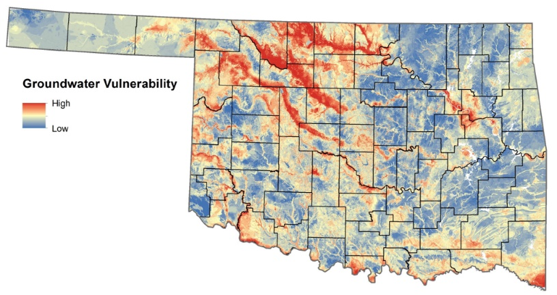
\includegraphics[width=1\linewidth]{img/DRASTIC} \caption{An example of a completed DRASTIC index for Oklahoma.}\label{fig:DRASTIC}
\end{figure}

~~~~~~A succesful DRASTIC+ index will not necesarrily correctly estimate the occurence of contamination, but should positively correlate with occurences. I will also test the sensitivity of DRASTIC+ accross all twenty tropical cyclones to estimate the range of vulnerability values over space and time. It will be of interest to investigate how physical vulnerability is dynamic over space versus time. I will quantify this by testing the index on a per-pixel basis over time and comparring the results.

~~~~~~Finally, I plan to investigate how `physical' vulnerabilty relates to vulnerability in a `socio-economic' sense. Census data will be used to tease out populations who are disproportionately affected by high `physical' vulnearbility. This will include quantification of well counts based on my previous work at EPA, income, education, and race.

\hypertarget{outcomes}{%
\chapter{Projected Outcomes}\label{outcomes}}

The research proposed here will yield valuable, quantitative understanding of the hydrogeologic cycle and how it is impacted by extreme precipitation events and land use/land cover patterns. I will add knowledge with regards to SM variance surrounding extreme precipitation events and its effects on available storage, rebound-ability of the landscape and thus contamination vulnerability. I will develop a method based on these concepts capable of providing forward and current estimates of groundwater vulnerability for the southeastern United States, which will use publicly available data. This method will be published as either a stand-alone product or an added variable to an existing weather or emergency response system such as the Short-term Prediction Research and Transition Center (SPoRT) real-time Land Information System. The societal relevance of this work includes the ability to pre-emptively plan for potential disaster response scenarios with knowledge of potential impacts based on up-to-date soil saturation characteristics and variable soil parameters such as conductivity and recharge. My proposed method will aid emergency management officials in identifying areas of potential impacts that may be underreported due to the ability of water contamination to go undetected without proper testing.

\hypertarget{timeline}{%
\chapter{Research Timeline}\label{timeline}}

This work is to be undertaken over two years. \textbf{Year} 1 will focus on establishing relationships between SM change and landscape variables such as hillslope and land cover, validation of SM measurements and conversion to DRASTIC variables with specific attention to validation using in-situ SM data. \textbf{Year 2} will be include model validation using storms where we have well testing records. I plan to present results in academic journals and at conferences throughout my research, particularly at the American Geophysical Union fall meeting and smaller conferences such as the Water Resources Research Institute. Publications are planned for the conversion of SMAP data into hydrogeological variables for groundwater modelling, temporal applications of an enhanced DRASTIC method and established relationships between SM variability and groundwater storage availability. Results and methods will also be made available via \href{AmurrayGeo.com/projects/cyclones/}{my website} where you can already view preliminary analyses. I also plan to monitor upcoming cyclone seasons for potential application testing. Our lab has been participating in long-term (2+ yr) monitoring efforts of dozens of surface and groundwater testing sites in the wake of Hurricane Matthew and Hurricane Florence.

\hypertarget{summary}{%
\chapter{Summary}\label{summary}}

This first-of-its-kind method will provide valuable insight into the effects of extreme precipitation derived from tropical cyclones on groundwater resources while leveraging cutting edge data and assimilation methods recently produced accross the fields of hydrology and remote sensing. The benefits to the population will be direct and will have the added value of promoting future development of earth-sensing satellites and sub-orbital airborne missions, specifically regarding SM. The necessary data for this work already exists and is freely available. My background in Geography and Remote Sensing gives me the necessary experience and capability to draw from and effectively utilize the various datasets this method will require. My three years of experience at EPA provided me with a thorough appreciation of the potential risks that groundwater contamination poses to human health. The timing of this research will also benefit work utilizing the SWOT (2021) and NISAR (2022) missions which will continue to evolve sensing capabilities of the water cycle, and may be applied to ongoing SM measurements using other methods such as NASA's GPM constellation satetlites and continued work downscaling SMAP. Finally, this work will enable better assessment and management of water quality, improving the capability to assess and respond to natural hazards and extreme events, and providing significant societal impact in the form of protecting human health.

  \bibliography{book.bib,packages.bib,journal.bib}

\end{document}
